%!TEX root = ../slides.tex
\section{Introduction}
\subsection{Motivation}
\begin{frame}{Research background}{Motivation}
\begin{figure}[tb]
  \centering
  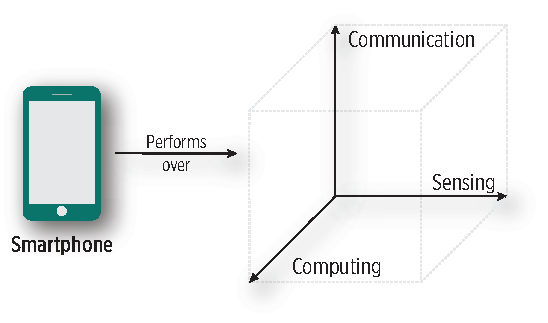
\includegraphics[width=0.4\textwidth]{vectors/smartphone-dimensions-v2}
  \caption{The advances in the communication, computing and sensing dimensions of mobile devices contribute to their acceptance by society~\cite{Islam2014}.}  
\end{figure}

\begin{block}{\small \textbf{Motivation}}
{
  \small
\begin{itemize}
  \item The sensing dimension enables \emph{context-awareness} in mobile devices, such as the smartphone.
  \item Battery advances are slower than those of other smartphone components~\cite{Kjaergaard2012}, growing 5-10\% yearly~\cite{Ma2012,Evarts2015}, a critical issue for the \textbf{mobile sensing applications}.
  % \item Battery advances are slower than those of other smartphone components~\cite{Kjaergaard2012}, growing 5-10\% yearly~\cite{Ma2012,Evarts2015}.
  % \item The energy constraint is critical for the continuous access to sensors required by \textbf{mobile sensing applications}. 
  \item Scientific efforts have been done for achieving the energy efficiency of the GPS location provider.
  \item The understanding of mobility could augment the location-awareness of the smartphone for many purposes, such as energy savings and the development of Mobility Based Services (MBSs).
  % \item As a high level of abstraction, mobility can be characterized as a sequence of frequently visited places (stay points).
\end{itemize}
}
\end{block}
\end{frame}

% \begin{frame}{Research background}{Motivation}
% \begin{block}{\small \textbf{Motivation}}
% {
%   \small
%    \begin{itemize}
%      \item For the sensing dimension, scientific efforts have been done for achieving the energy efficiency of the GPS location provider.
%      \item The understanding of mobility could augment the location-awareness of the smartphone for many purposes, such as energy savings and the development of Mobility Based Services (MBSs).
%      \item As a high level of abstraction, mobility can be characterized as a sequence of frequently visited places (a.k.a. stay points).
% \end{itemize}
% }
% \end{block}
% \end{frame}

\subsection{Research background}
%\subsection{Problem statement}
\begin{frame}{Research background}{Problem statement}
\small
\vspace{-0.5cm}
\begin{itemize}
  \item The understanding of mobility is possible at different spatial-temporal scales:
\end{itemize}

\begin{exampleblock}{\small \textbf{Fine-grain mobility patterns identification}}
 \begin{itemize}
    \item They refer to the transportation mode employed by user when moving between stay points.
    \item Given a set of values $\mathcal{V} = v_{acc~1},v_{acc~2},\ldots,v_{acc~n}$ obtained from accelerometer in the time interval $[t_1,t_2]$, identify fine-grain mobility information:
\begin{equation*}
  \text{\textbf{FineGrainMobilityIdentifier}}(\mathcal{V}) \rightarrow p_S \in \{ \text{static, walking, biking, vehicle} \}
\end{equation*}
with each $v_{acc~i} \in \mathcal{V}$ composed as $\langle acc_x,acc_y,acc_z,t \rangle$.
  \end{itemize} 
\end{exampleblock}

\begin{exampleblock}{\small \textbf{Coarse-grain mobility patterns identification}}
 \begin{itemize}
   \item They refer to motion at a large spatial scale related to user visiting stay points.
   \item \sloppy Given a set of values $\mathcal{V} = v_{gps~1},v_{gps~2},\ldots,v_{gps~n}$ obtained from GPS location provider in time interval $[t_1,t_2]$, identify coarse-grain mobility information:
\begin{equation*}
    \text{\textbf{CoarseGrainMobilityIdentifier}}(\mathcal{V}) \rightarrow p_S \in \{ \text{new stay point, arrival, departure} \}
\end{equation*}
with each $v_{gps~i} \in \mathcal{V}$ composed associated $\langle lat, lon, t \rangle$.
 \end{itemize}
\end{exampleblock}
\end{frame}


\begin{frame}{Research background}{Problem statement}
\small

\begin{exampleblock}{\small \textbf{Sensors sampling adaptation}}
\begin{itemize}
\item Given a set of coarse and fine-grain mobility patterns $\mathcal{P} = \{ p_{S_1}, p_{S_2}, \ldots, p_{S_n} \}$, and accuracy requirements of mobile app $req_{accuracy}$, implement a sampling policy for the adaptive duty cycling of sensors while reducing energy consumption:
\begin{equation*}
  \text{\textbf{PolicyGeneration}}( \mathcal{P}, req_{accuracy}) \longrightarrow{} \mathcal{S}_{conf}
\end{equation*}
where $\mathcal{S}_{conf} \rightarrow s, \mathcal{T}_{real}$ represents the sampling $\mathcal{T}_{real}$ that must be implemented for sensor $s$.
The $req_{accuracy}$ refers to the granularity of GPS sampling.
\end{itemize}
\end{exampleblock}

\begin{figure}[tb]
  \centering
  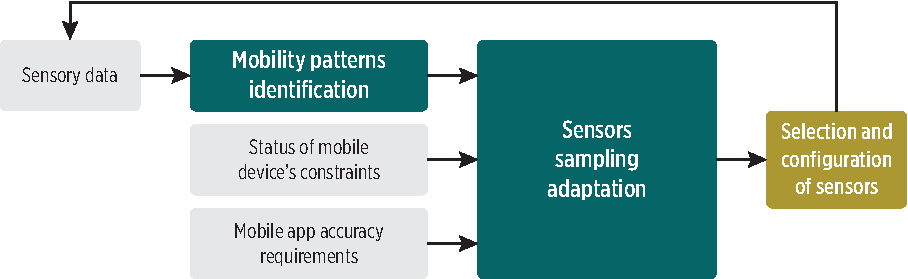
\includegraphics[width=0.7\textwidth]{vectors/problems-incorporation-v2}
  \caption{Interaction between problems.}
\end{figure}
\end{frame}

% \subsection{Hypothesis}
\begin{frame}{Research background}{Hypothesis}
\small
\begin{block}{\small \textbf{Hypothesis}}
\renewcommand{\baselinestretch}{1.4}
\begin{itemize}
  \item The energy consumption of continuous and extended location tracking could be reduced by means of a cognitive dynamic system that learns an expanded spatial-time model from mobility events detected from sensors data and that employs such model in a cognitive controller for dynamically adapting GPS sampling rate through sampling policies tailored to current mobility state.
\end{itemize}
\end{block}
\end{frame}


% \subsection{Objectives}
\begin{frame}{Research background}{Objectives}
\small
\begin{block}{\small \textbf{Main objective}}
\begin{itemize}
  \item To reduce the energy consumption of mobile sensing apps, which perform continuous sensor sampling, through self-adapting power-aware policies generated from context information obtained from sensors data.
\end{itemize}
\end{block}

\begin{block}{\small \textbf{Particular objectives}}
\begin{itemize}
  \item To detect mobility patterns from context information obtained from an inertial sensor (accelerometer) and location provider (GPS).
  \item To generate an accurate representation of detected patterns for summarizing user mobility.
  \item To dynamically adapt GPS sampling rate by means of a cognitive controller that employs the learned mobility representation and accuracy requirements for implementing power-aware sampling policies.
  \item To ease the development of mobile sensing applications that require user location tracking, i.e., LBSs and MBSs, isolating the complexity of sensors access and the associated efficient energy management.
\end{itemize}
\end{block}
\end{frame}



% \subsection{Methodology}
\begin{frame}{Research background}{Methodology}
\small
\begin{block}{\small \textbf{Methodology}}
\begin{enumerate}
  \item \textbf{Revision of state of the art power-aware sensing techniques.}
  \item \textbf{Formal definition and selection of mobility patterns to be identified.}
  \item \textbf{Research on algorithms for detecting mobility patterns.}
  \item \textbf{Design of the \emph{Mobility Events Detector}.}
  \item \textbf{Design of adaptive policies for energy efficient usage of sensors.}
  \item \textbf{Design of the Cognitive Controller.}
  \item \textbf{Development of a middleware involving the \emph{Mobility Events Detector} and the Cognitive Controller for the Android platform.}
  \item Experimentation in terms of spatial-time accuracy and energy efficiency.
\end{enumerate}
\end{block}
\end{frame}
